\mode<article>{
\chapter{SystemC Basics \& Cycle Level Modeling with SystemC}
}

\mode<presentation>{
\part{SystemC Basics \& Cycle Level Modeling with SystemC}
}

\mode<presentation>{
\begin{frame}
	\frametitle{\small VP3: SystemC Basic \& Cycle Level Modeling with SystemC}
	Outline
	\begin{itemize}
		\item<1->Principles
		\begin{itemize}
			\item<1->Hierarchical decomposition of the system
			\item<1->Model of computation \& Process scheduling
		\end{itemize}
		\item<1->The SystemC syntax
		\begin{itemize}
			\item<1->The modules
			\item<1->The ports \& signals
			\item<1->The processes
			\item<1->Building the simulator
			\item<1->Initialization phase
		\end{itemize}
		\item<1->Exercise
		\item<1->Futher more abstraction
		\begin{itemize}
			\item<1->Dynamic sensitivity \& Events
			\item<1->Abstract communication channels
		\end{itemize}
	\end{itemize}
\end{frame}
}

\mode<article>{
In this chapter, you will learn the basics of SystemC, and especially how to use the basic syntax of SystemC to write cycle level models.
}

\section{Principles}

\subsection{Hierarchical decomposition of the system}

\mode<presentation>{

\begin{frame}
	\frametitle{Hierarchical decomposition of the system}
	\begin{itemize}
		\item<1->SystemC inherited cycle level modeling style from previous hardware level description languages such as VHDL and Verilog
		\item<1->SystemC provides the user with C++ classes to model:
		\begin{itemize}
			\item<1->Hardware/Software components: Modules
			\item<1->Communications: Ports, Signals
			\item<1->Component Behavior: Processes
		\end{itemize}
		\item<1->A simulator of the system is an assembly of SystemC modules
		\item<1->Main simulation loop is within the SystemC library
		\item<1->User defines a "sensitivity list" for each process to enable SystemC fire/schedule processes
	\end{itemize}
\end{frame}
\begin{frame}
	\frametitle{Example of system}
	\begin{figure}[h]
		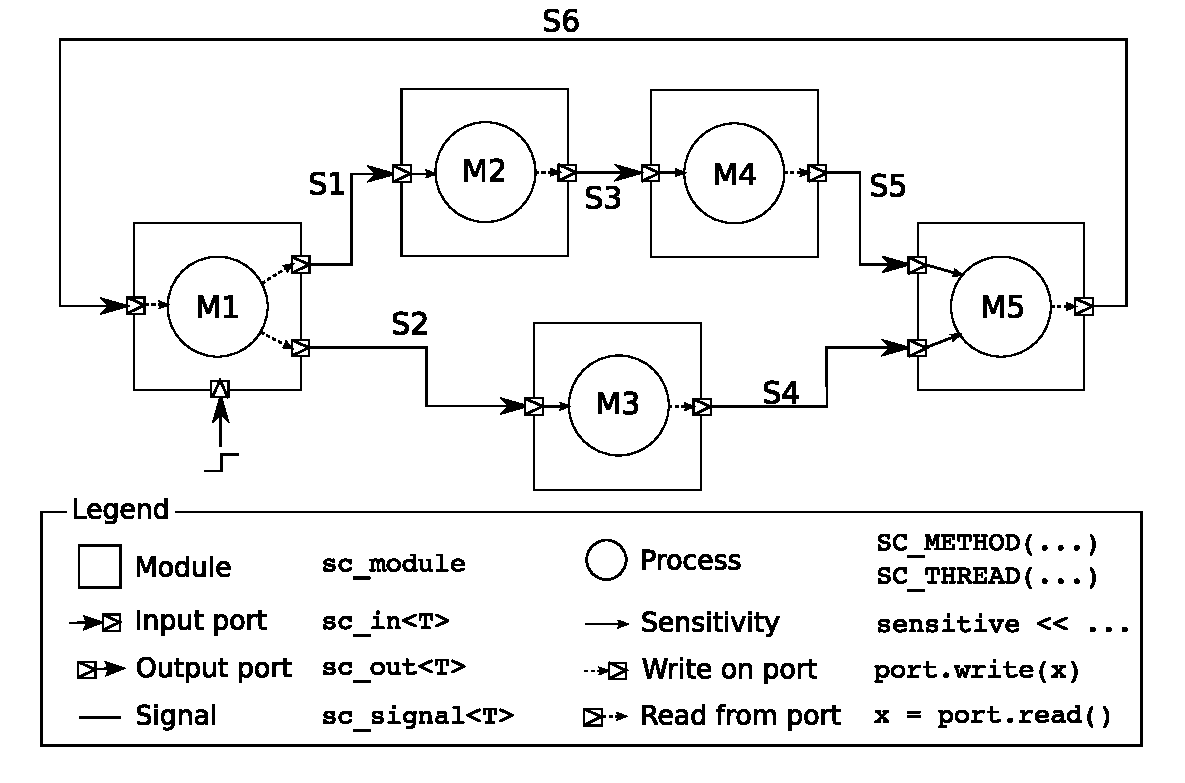
\includegraphics[width=\textwidth]{systemc_cycle/systemc_example.pdf}
	\end{figure}
\end{frame}
}

\mode<article>{

In SystemC, the system is hierarchically decomposed in components, called modules, for instance a processor, a cache, a functional unit, or any other circuit.
These modules communicate each other thanks to links between module ports, called signals.
The behavior of each module, that is reading the input signals, computing, and generating the output signals is performed in one or several processes.
The list of a process input signals that need regenerating the process output signals is called the sensitivity list.

For instance, Figure~\ref{fig:systemc_example} shows a system with several modules. The system is composed of 5 modules with one process each. Process~P1 of module~M1 reads signal~S6, and produces signals~S1~and~S2.
The sensitivity list of process~P1 only contains the clock rising edge.
Process~P5 of module~M5 has signals~S4~and~S5 in its sensitivity list, and produces signal~S6.

\begin{figure}[!h]
	\begin{center}
		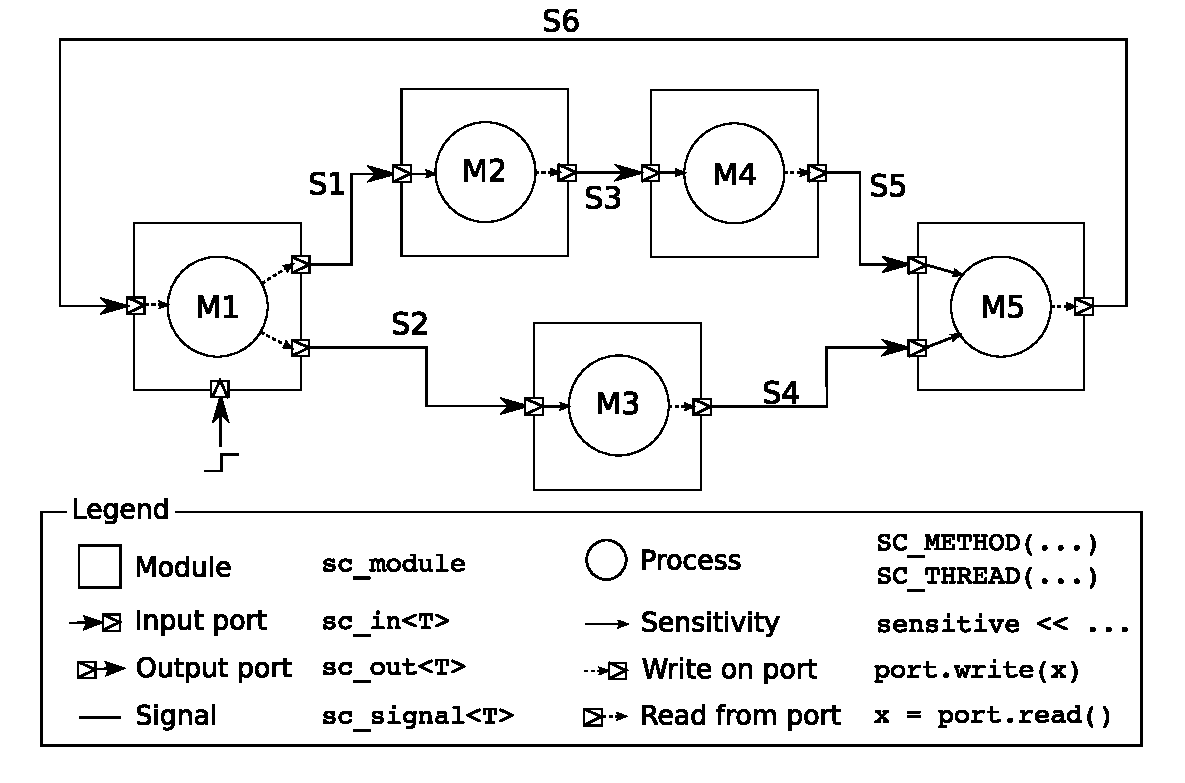
\includegraphics[width=\textwidth]{systemc_cycle/systemc_example.pdf}
	\end{center}
	\caption{Example of a system.}
	\label{fig:systemc_example}
\end{figure}
}

\subsection{Model of computation and process scheduling}

\mode<presentation>{
	\begin{frame}
		\frametitle{Model of computation}
		\begin{itemize}
			\item<1->Charastetistic of hardware systems:
			\begin{itemize}
				\item<1->Signals are continuously computed (1)
				\item<1->Naturally parallel (2)
			\end{itemize}
			\item<1->But:
			\begin{itemize}
				\item<1->SystemC can model parallelism
				\item<1->Host machine execution model is sequential
				\item<1->Underlying C++ language is sequential
				\item<1->Simulation behavior should not depend on process scheduling
			\end{itemize}
			\item<1->(1) $\rightarrow$ SystemC model of computation: Discrete event
			\item<1->(2) $\rightarrow$ SystemC relies on an evaluate/update mechanism
		\end{itemize}
	\end{frame}

	\begin{frame}
		\frametitle{Process scheduling}
		\begin{figure}[!h]
			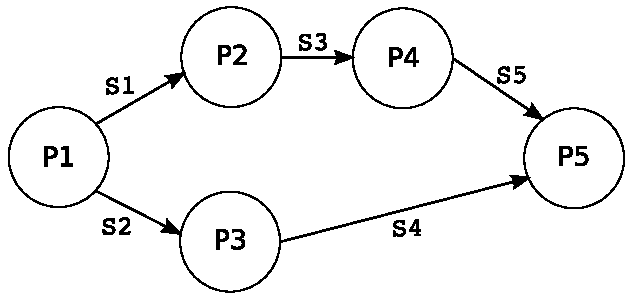
\includegraphics[width=7cm]{systemc_cycle/dependency_graph.pdf}
			\newline
			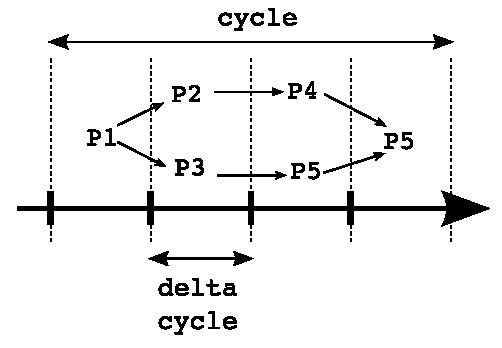
\includegraphics[width=7cm]{systemc_cycle/schedule_example.pdf}
		\end{figure}
	\end{frame}

}

\mode<article>{

The SystemC simulation engine dynamically schedules the processes.
SystemC uses the evaluate/update paradigm.
SystemC wakes up a process whenever at least one signal in its sensitivity list has changed, in order to regenerate the output signals of the module.
When a process writes on a signal, the value is not immediately available on the signal. It is only after all processes have been waken up, that the signals which have changed are updated, that is propagated.
Their new values are then available for all the processes.
This way, the order in which processes wake up do not determine the simulation result.
Each evaluate/update cycle is called a delta cycle.

The simulation of one clock cycle is composed of several delta cycles.
At the beginning of the clock cycle, the processes which are sensitive to the clock are waken up in "parallel", that is at the same delta cycle, and the signals are then propagated.
The signals that have changed, wake up other processes, and so on until there is no more processes to wake up.
Thus, one simulated clock cycle terminates when the system became stable.
The number of delta cycles for a simulated clock cycle is not known in advance.

For instance, for the system of Figure~\ref{fig:systemc_example}, Figure~\ref{fig:schedule_example} shows the graph of processes of the system where the nodes are the processes, and the edges are the signals that changes.
Process~P1 is sensitive to the clock rising edge. Process~P1 thus wakes up first, and update signals~S1~and~S2. Signals~S1~and~S2 are propagated. Processes~P2~and~P3 wake up because they are sensitive to respectively signals~S1~and~S2, and these processes updates signals~S5~and~S6.
Signals~S5~and~S6 are propagated. Process~P5 wakes up because it is sensitive to signal~S5. Signal~S6 is propagated but does not wake up any process, and the simulated clock cycle is thus finished.
The simulation engine advance the system clock, and so on.
The simulation of that clock cycle taked 4 delta cycles. Note that the processes do not necessarily wake up only one time per simulated clock cycle.
For instance, Process~P5 woke twice: one time because of signal~S4 updated by process~P4, and one time because of signal~S5 updated by process~P3.

\begin{figure}[!h]
	\begin{minipage}{8.0cm}
	\begin{center}
			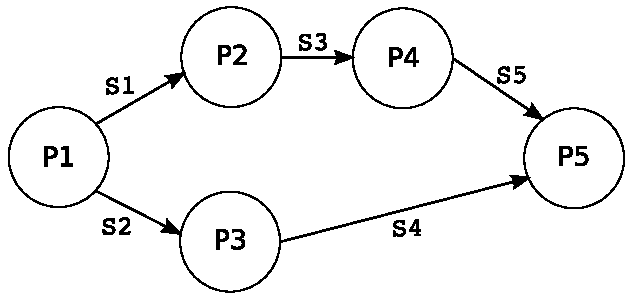
\includegraphics[width=8cm]{systemc_cycle/dependency_graph.pdf}
	\end{center}
	\end{minipage}
	\begin{minipage}{8.0cm}
	\begin{center}
			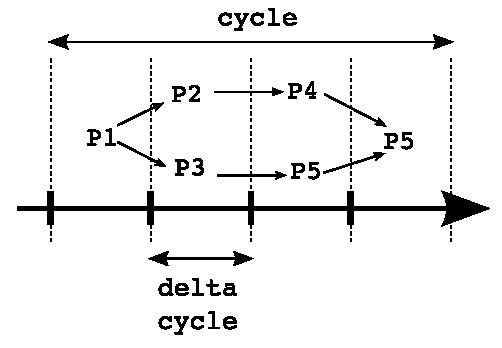
\includegraphics[width=8cm]{systemc_cycle/schedule_example.pdf}
	\end{center}
	\end{minipage}
	\caption{Example of SystemC process schedule.}
	\label{fig:schedule_example}
\end{figure}
}

\section{The SystemC syntax}

\subsection{The modules}

\mode<presentation>{
	\begin{frame}
		\frametitle{The modules}
		\begin{itemize}
			\item<1->Module: A C++ object modeling a hardware/software component
			\item<1->SystemC provides a C++ base class: \texttt{sc\_module}
			\item<1->User's modules derive from \texttt{sc\_module}
			\item<1->Each module has a unique name of type \texttt{sc\_module\_name}
			\item<1->
			\begin{block}{User's module definition looks like:}
				\lstinputlisting{systemc_cycle/module_definition.cc}
			\end{block}
		\end{itemize}
	\end{frame}
}

\mode<article>{
The base class \texttt{sc\_module} is an object representing a simulator module.
The user defines a new module class by derivating class \texttt{sc\_module}.
}

\subsection{The ports and signals }

\mode<presentation>{
	\begin{frame}
		\frametitle{The ports}
		\begin{itemize}
			\item<1->Port: A module communicates with the world using it
			\item<1->It's a module public member of type \texttt{sc\_in<T>} or \texttt{sc\_out<T>}
			\item<1->\texttt{T} is the data type transmitted through the port: e.g. int, double \ldots
			\item<1->
			\begin{block}{Module reads/writes ports just like normal C++ variables :}
				\lstinputlisting{systemc_cycle/port_access.cc}
			\end{block}
		\end{itemize}
	\end{frame}

	\begin{frame}
		\frametitle{The signals}
		\begin{itemize}
			\item<1->Signal: similar to a wire
			\item<1->Ports are bound to signals to assemble modules
			\item<1->It's a C++ variable of type \texttt{sc\_signal<T>}
			\item<1->Like ports, \texttt{T} is the data type transmitted over the signal: e.g. int, double \ldots
			\item<1->
			\begin{block}{Ports are bound to signal using operator () of ports:}
				\lstinputlisting{systemc_cycle/port_signal_binding.cc}
			\end{block}
		\end{itemize}
	\end{frame}
}

\mode<article>{
Each port is a public member of the module class.
The input ports are of type \texttt{sc\_in<type>}, where \texttt{type} is the type of the data which is transmitted through those ports.
To declare a signal, the user instantiates an object of class~\texttt{sc\_signal<type>}, where \texttt{type} is the type of the data which is transmitted over the signal.
SystemC only accepts ports and signals which types have operator \texttt{==} (comparison operator) and operator \texttt{<<} of \texttt{ostream} available.
These operators are useful because SystemC needs to check whever a signal value has changed or to display the content of a signal.
The clock, of type \texttt{sc\_clock} is a special signal that the SystemC simulation engine automatically waves: it can be bound to a special clock port of type \texttt{sc\_in\_clk}.
}

\subsection{The processes}

\mode<presentation>{
	\begin{frame}
		\frametitle{The processes}
		\begin{itemize}
			\item<1->Process: A public member method of the module class
			\begin{itemize}
				\item<1->A simple C++ method: \texttt{SC\_METHOD}.
				SystemC kernel calls the method each time process is scheduled
				\vspace{-0.5cm}
				\begin{figure}[h]
					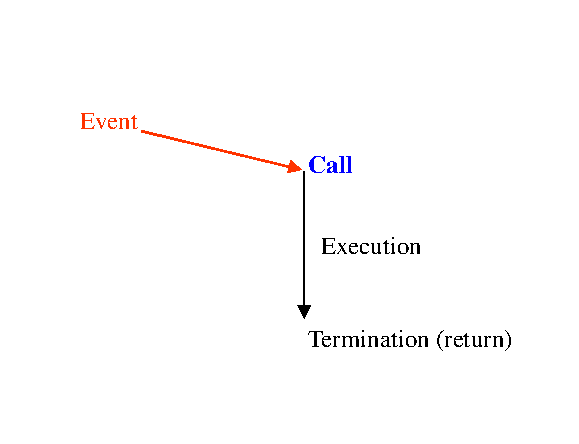
\includegraphics[width=4.0cm]{systemc_cycle/method.pdf}
				\end{figure}
				\vspace{-0.5cm}
				\item<1->A thread: \texttt{SC\_THREAD} or \texttt{SC\_CTHREAD}
				SystemC kernel switches to the thread each time process is scheduled
				\vspace{-0.5cm}
				\begin{figure}[h]
					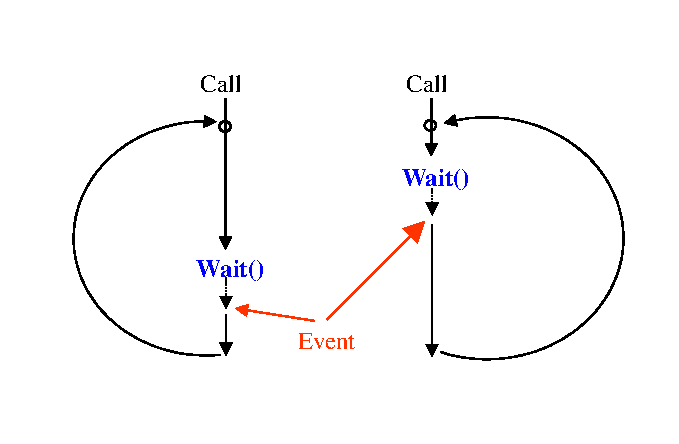
\includegraphics[width=4.0cm]{systemc_cycle/threads.pdf}
				\end{figure}
			\end{itemize}
		\end{itemize}
	\end{frame}

	\begin{frame}
		\frametitle{SC\_METHOD processes}
		\begin{block}{Definition of an SC\_METHOD process in module constructor:}
			\lstinputlisting{systemc_cycle/sc_method_definition.cc}
		\end{block}
	\end{frame}

	\begin{frame}
		\frametitle{SC\_THREAD processes}
		\begin{block}{Definition of an SC\_THREAD process in module constructor:}
			\lstinputlisting{systemc_cycle/sc_thread_definition.cc}
		\end{block}
	\end{frame}

	\begin{frame}
		\frametitle{SC\_CTHREAD processes}
		\begin{block}{Definition of an SC\_CTHREAD process in module constructor:}
			\lstinputlisting{systemc_cycle/sc_cthread_definition.cc}
		\end{block}
	\end{frame}
}

\mode<article>{
The processes model the module behavior, and are implemented in some module methods.
These methods are either invoked by a simple method call, see Figure~\ref{fig:process}a, or by a context switch, see Figure~\ref{fig:process}b.
The former is known as a \texttt{SC\_METHOD} process, the latter is known as a thread process (actually a user thread).
A thread process never finishes: it's typically an infinite loop with some calls to SystemC primitive \texttt{wait}.
This primitive leaves control to the main thread, that is the SystemC engine.
Figure~\ref{fig:basic_wait} shows the possible use of the wait primitive.

\begin{figure}[!h]
\begin{center}
\lstinputlisting{systemc_cycle/basic_wait.cc}
\end{center}
\vspace{-0.5cm}
\caption{\label{fig:basic_wait} Example of use of the wait primitive.}
\end{figure}

A SystemC thread can be of two types: \texttt{SC\_THREAD} or \texttt{SC\_CTHREAD}.
An \texttt{SC\_CTHREAD} is only sensisitive to the clock whereas an \texttt{SC\_THREAD} is sensitive to any kind of signal.
SystemC has three C++ macro to declare in the module constructor a C++ member method as a SystemC process: \texttt{SC\_METHOD(\ldots)}, \texttt{SC\_THREAD(\ldots)}, \texttt{SC\_CTHREAD(\ldots)}.
The sensitive list of a process is represented by an object, called \texttt{sensitive}: \texttt{sensitive << port} adds a port, and the signal bound to that port, to the sensitive list of a process; \texttt{sensitive << port.pos()} and \texttt{sensitive << port.neg()} respectively adds the clock port (of type \texttt{sc\_in\_clk}) rising/falling edge to the sensitive list of a process.
\texttt{sensitive << signal} is also a legal statement.

Figure~\ref{fig:systemc_example_impl} shows the implementation of modules~M1~and~M5 for the system of Figure~\ref{fig:systemc_example}.
The classes of modules~M1~and~M5 derive from class \texttt{sc\_module}. Modules~M1~and~M5 declare three ports each.
For instance, in module~M1, \texttt{clock} is the port connected to the clock signal, \texttt{input} is an input port where one can read an integer, and \texttt{output[i]} an output port where one can write an integer.
Module~M1 declares a process of type \texttt{SC\_METHOD} which is sensitive to the clock rising edge.
Module~M5 declares a process of type \texttt{SC\_METHOD} which is sensitive to ports \texttt{input[i]}.
In module~M1, Process~P1 reads port \texttt{input}, update the internal \texttt{state} of module~M1, and write on ports \texttt{output[i]}.
In module~M5, Process~P5 reads ports \texttt{input[i]}, computes a new value, and write the result on port \texttt{output}.

\begin{figure}[!h]
\begin{minipage}{\textwidth}
\begin{minipage}{7.0cm}
\begin{center}
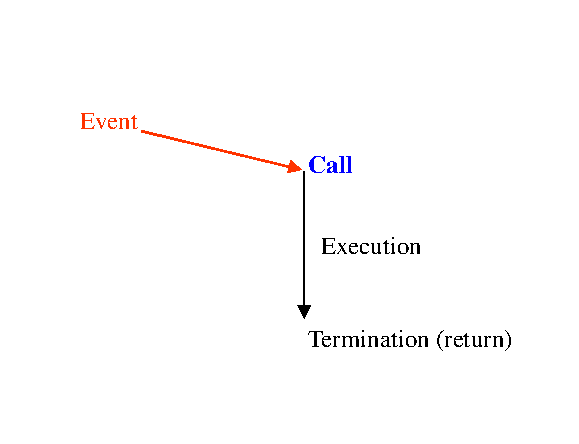
\includegraphics[width=7.0cm]{systemc_cycle/method.pdf}
\end{center}
\end{minipage}
\begin{minipage}{7.0cm}
\begin{center}
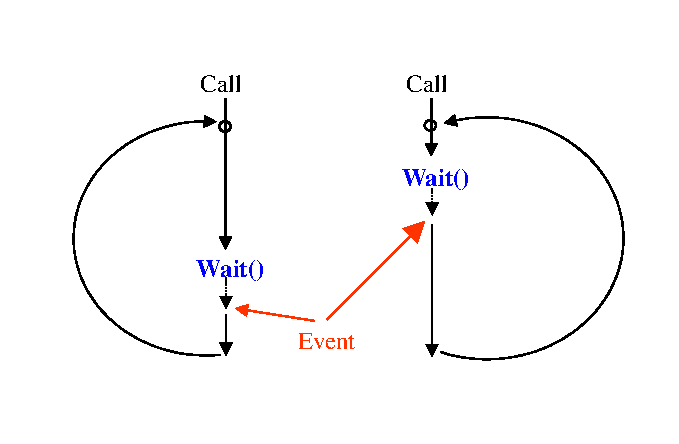
\includegraphics[width=7.0cm]{systemc_cycle/threads.pdf}
\end{center}
\end{minipage} 
\begin{minipage}{7.0cm}
\begin{center}
(a)
\end{center}
\end{minipage}
\begin{minipage}{7.0cm}
\begin{center}
(b)
\end{center}
\end{minipage}
\caption{\label{fig:process} \small (a) \texttt{SC\_METHOD} process; (b) \texttt{SC\_THREAD} process.}
\end{minipage}
\end{figure}
}

\subsection{Building the simulator}

\mode<presentation>{
	\begin{frame}
		\frametitle{Building the simulator: an example}
		\lstinputlisting{systemc_cycle/connecting.cc}
	\end{frame}
}

\mode<article>{
Once every modules of the system have been developped, they can assembled to get a complete executable model.
Each modules ($M_i, 1 \leq i \leq 5$) and signals (clock, $S_j, 1 \leq j \leq 6$) shall be instantiated and connected using module ports.
The connections between ports and signals is usually called a \textbf{Netlist}.
SystemC defines special C++ operators for ports and signals to bind ports and signals: \texttt{port(signal)} actually bind a port and a signal.
Figure~\ref{fig:connecting} shows how this can be used to build the netlist of the system.
In this implementation a clock with a period of 10 nanoseconds has been instantiated.
The simulation is run for 1000 nanoseconds by invoking SystemC primitive \texttt{sc\_start}.

\begin{figure}[!h]
\begin{center}
\lstinputlisting{systemc_cycle/systemc_example.cc}
\end{center}
\vspace{-0.5cm}
\caption{\label{fig:systemc_example_impl} Implementation of modules~M1~and~M5 for system of Figure~\ref{fig:systemc_example}}
\end{figure}

\begin{figure}[!h]
\begin{center}
\lstinputlisting{systemc_cycle/connecting.cc}
\end{center}
\vspace{-0.5cm}
\caption{\label{fig:connecting} Netlist implementation for system of Figure~\ref{fig:systemc_example}}
\end{figure}
}

\subsection{Initialization phase}

\mode<presentation>{
	\begin{frame}
	\frametitle{Initialization phase}
		\begin{block}{Initial delta cycles}
		At initialization phase, SystemC calls every processes, and simulates one or more delta cycles.
		This initialization ends when no more signals have changed, and thus the system is stable.
		\end{block}
	\end{frame}
}

\mode<article>{
At initialization phase, SystemC calls every processes, and simulates one or more delta cycles.
This initilization ends when no more signals have changed, and thus the system is stable.
}

\section{Exercise}
\label{clm_exercise}

\mode<presentation>{
	\begin{frame}
		\frametitle{Exercise 1}
		\begin{figure}[h]
			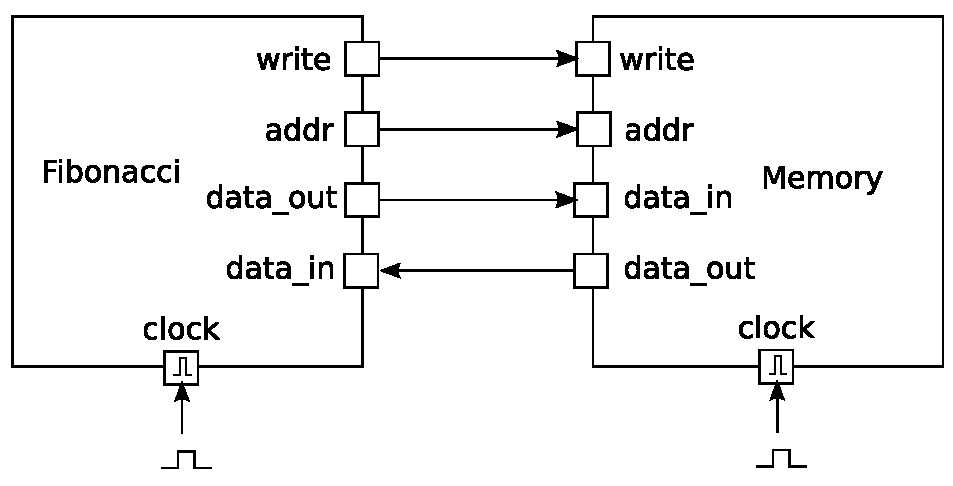
\includegraphics[width=9.0cm]{systemc_cycle/fibonacci.pdf}
		\end{figure}
	\end{frame}

	\begin{frame}
		\frametitle{Exercise 2}
		\begin{figure}[h]
			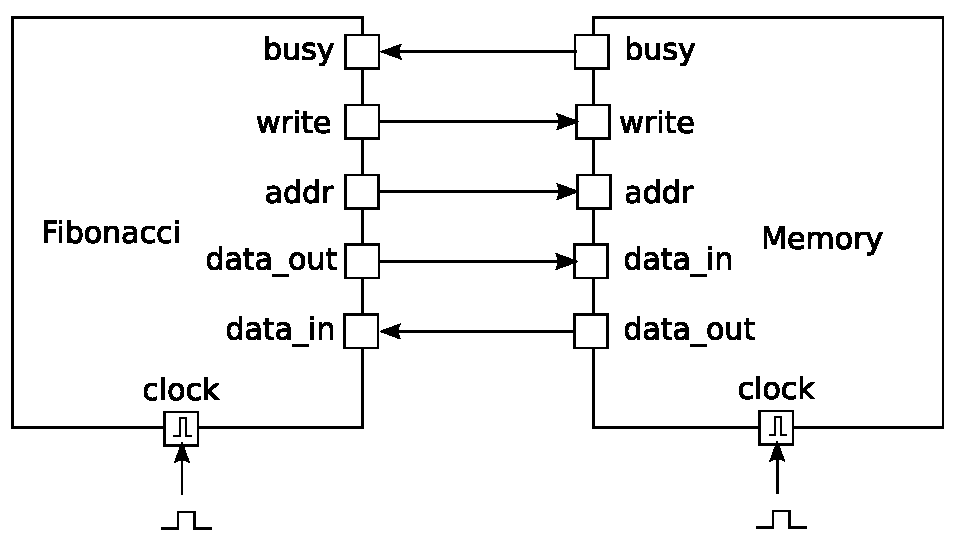
\includegraphics[width=9.0cm]{systemc_cycle/fibonacci_with_wait_states.pdf}
		\end{figure}
	\end{frame}
}

\mode<article>{
The goal of these exercises is to highlight the SystemC features which allow to develop cycle level models.
In this scope, we will consider the system of Figure~\ref{fig:cycle_level_fibonacci}.
It is composed of two modules: a Fibonacci module and a memory module.
The Fibonacci module implements the recursive version of Fibonacci algorithm, see Figure~\ref{fig:fibonacci_cpp_program}.
The Fibonacci module will use the memory module as a stack to transmit argument \texttt{n} and return the result of the computation to the caller.
To do so, you will need a stack pointer (i.e. an address) in the Fibonacci module which points to the top of the stack.

\begin{figure}[h]
	\begin{center}
		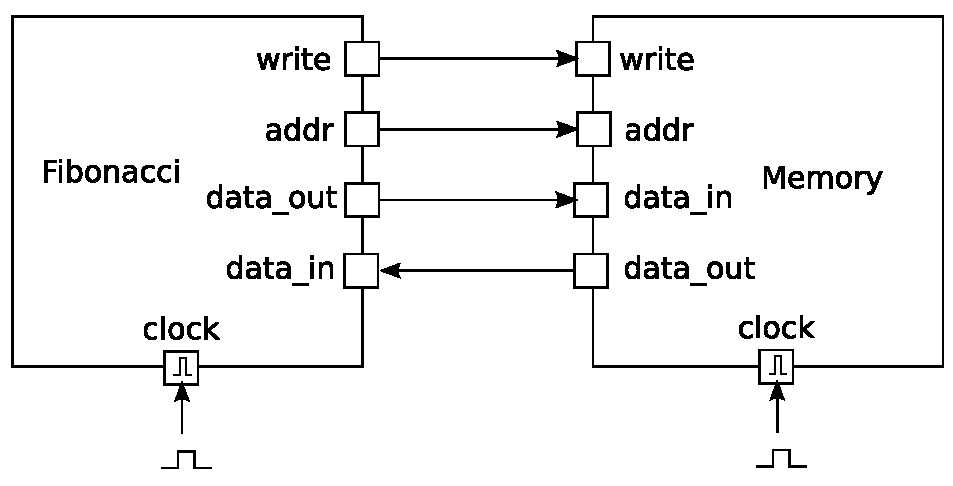
\includegraphics[width=12.0cm]{systemc_cycle/fibonacci.pdf}
	\end{center}
	\caption{Cycle level model of Fibonacci.}
	\label{fig:cycle_level_fibonacci}
\end{figure}

As a first approximation, we consider that:
\begin{itemize}
\item Each step of the Fibonacci algorithm, i.e. the additioner, takes one cycle latency.
\item A memory write takes a full clock cycle (one clock cycle latency).
\item A memory access has no wait states: the result of a read is available before the end of the clock cycle.
\end{itemize}
}

\subsection{Module interface definitions}

\mode<article>{
Define the module interface for modules Fibonacci and Memory, and more precisely:
\begin{itemize}
\item Define the modules, i.e. the C++ classes
\item Define the ports as public member of the module class
\item Define the module constructor
\end{itemize}

}

\subsection{Module connection}

\mode<article>{
Instantiate and connect the two modules:
\begin{itemize}
\item Define an \texttt{sc\_main} (C++ main works too)
\item Define the signals
\item Instantiate the modules
\item Bind the module ports to the signals
\end{itemize}
}

\subsection{Behavior implementation}

\mode<article>{
Implement the behavior of module Memory and Fibonacci.
\begin{itemize}
\item Define which processes you need and their role
\item Declare these processes (in the module constructor) to the SystemC kernel using macros \texttt{SC\_METHOD}, \texttt{SC\_THREAD}, \texttt{SC\_CTHREAD}
\item Fill in the sensitive list of each process
\item Implement the processes
\end{itemize}
}

\subsection{Adding some wait states}

\mode<article>{
As a second approximation, we consider that:
\begin{itemize}
\item A memory access has wait states: writes take more than one cycle; the result of a read is not available before the end of the clock cycle; and memory requires additional clock cycles before the result is actually available on port \texttt{data\_out}.
\end{itemize}

Signal \texttt{busy} has been introduced. Memory asserts Signal \texttt{busy} to indicate that it requires additional clock cycle to perform the requested operation, see Figure~\ref{fig:cycle_level_fibonacci_with_wait_states}.
Once the data is available on port \texttt{data\_out}, memory deasserts signal \texttt{busy}.
Modify your simulator to support memory wait states.

\begin{figure}[!h]
	\begin{center}
		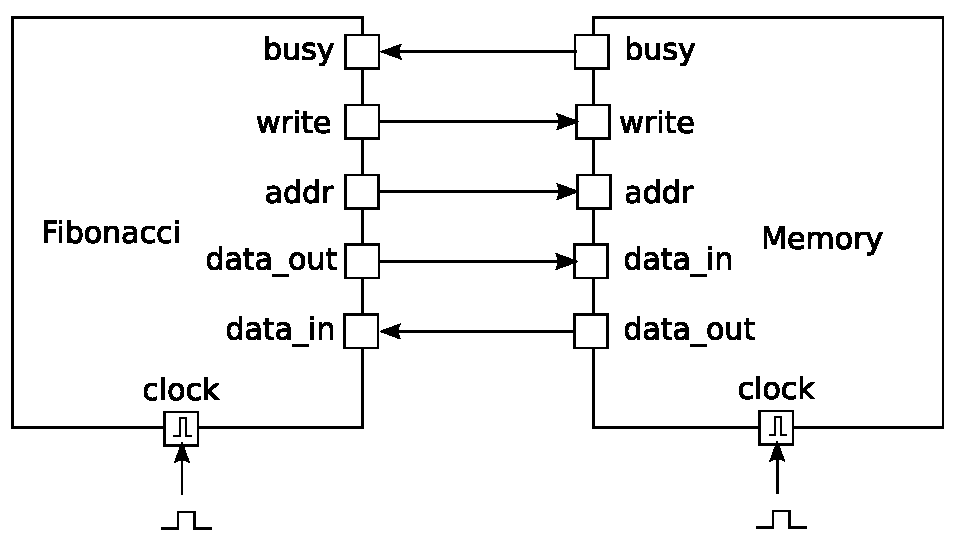
\includegraphics[width=12.0cm]{systemc_cycle/fibonacci_with_wait_states.pdf}
	\end{center}
	\caption{Cycle level model of Fibonacci with memory wait states.}
	\label{fig:cycle_level_fibonacci_with_wait_states}
\end{figure}
}

\section{A step further more abstraction}

\mode<presentation>{
	\begin{frame}
		\frametitle{A step further more abstraction}
		\begin{itemize}
			\item<1->SystemC basic syntax inherited from SystemC 1.x: only cycle level modeling
			\item<1->Lake of some intermediate steps between:
			\begin{itemize}
				\item<1->The specifications
				\item<1->The cycle accurate model 
			\end{itemize}
			\item<1->SystemC 2.x $\rightarrow$ Foundation to allow higher abstraction levels
		\end{itemize}
	\end{frame}
}

\mode<article>{
Recent versions of SystemC have introduced support for dynamic sensitivity list, events, and communication channels.
This was the first step toward more abstract modeling styles such as transaction level modeling (TLM).
}

\subsection{Dynamic sensitivity list \& Events}

\mode<presentation>{
	\begin{frame}
		\frametitle{Dynamic sensitivity list \& Events}
		\begin{block}{Dynamic sensitivity}
			"Ability to define at simulation time the events that makes a SystemC process wake up"
		\end{block}
		To be opposed to
		\begin{block}{Static sensitivity}
			"Ability to define at elaboration time (i.e. in module constructor) the sensitivity list"
		\end{block}

		SystemC 2.x introduced events and the ability for a process to wake up when an event is notified
	\end{frame}

	\begin{frame}
		\frametitle{Events and extended wait primitive}
		\begin{figure}[h]
			\lstinputlisting{systemc_cycle/advanced_wait.cc}
		\end{figure}
		\begin{figure}[h]
			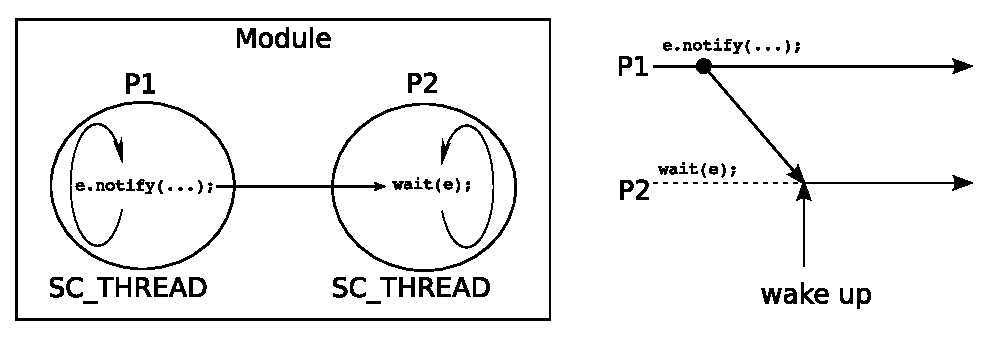
\includegraphics[width=8.0cm]{systemc_cycle/dynamic_sensitivity.pdf}
		\end{figure}
	\end{frame}
}

\mode<article>{
Dynamic sensitivity is the ability to define at simulation time the events that makes a SystemC process wake up.
It has to be opposed to static sensitivity which only allows the user to define the sensitivity list at elaboration time (i.e. in the constructor).
A new class \texttt{sc\_event} has been introduced, and the usage of the SystemC \texttt{wait} primitive has been extended to provide such a mechanism, see Figure~\ref{fig:advanced_wait}.

\begin{figure}[h]
\begin{center}
\lstinputlisting{systemc_cycle/advanced_wait.cc}
\end{center}
\vspace{-0.5cm}
\caption{\label{fig:advanced_wait} Example of use of the extended wait primitive.}
\end{figure}

Figure~\ref{fig:dynamic_sensitivity} shows the use of dynamic sensitivity. Process~P2 waits on event e. Process~P1 notify event e which make \texttt{wait} to return and Process~P2 wake up.

\begin{figure}[h]
	\begin{center}
		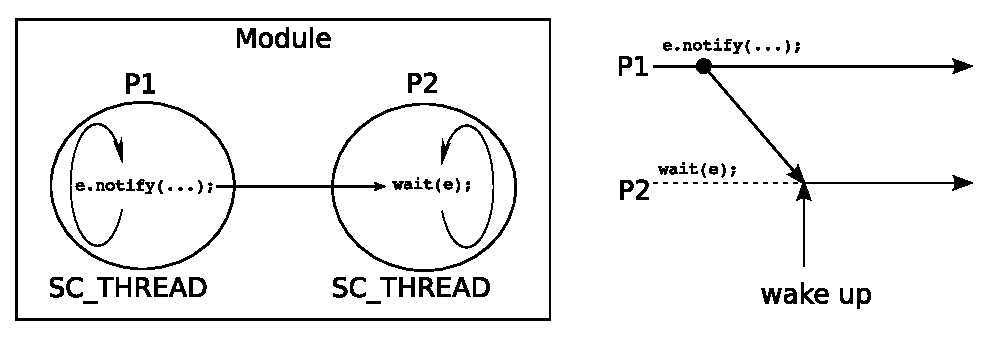
\includegraphics[width=10.0cm]{systemc_cycle/dynamic_sensitivity.pdf}
	\end{center}
	\vspace{-0.5cm}
	\caption{\label{fig:dynamic_sensitivity} Dynamic sensitivity.}
\end{figure}

}

\subsection{Dynamic Processes}

\mode<presentation>{
	\begin{frame}
		\frametitle{Dynamic Processes}
		\begin{itemize}
			\item<1->Hardware is static, thus corresponding SystemC process are created at elaboration time
			\item<1->Problem: Modeling dynamic software processes?
			\item<2->SystemC 2.0 introduces spawning threads at simulation time:
			\begin{itemize}
				\item<3->\texttt{sc\_spawn} \ldots
			\end{itemize}
		\end{itemize}
	\end{frame}
	\begin{frame}
		\frametitle{Dynamic Process Example}

		\begin{figure}[h]
			\lstinputlisting{systemc_cycle/dynamic_process.cc}
		\end{figure}
		
	\end{frame}
}

\mode<article>{

In earlier version of SystemC, processes were defined only at elaboration time in module constructor.
The main reason of that limitation is that hardware is mostly static or the number of pieces of hardware is easily defined at design.
The needs for modeling dynamic software processes, i.e. spawning processes at simulation time, has been addressed by later versions of SystemC by introducing a primitive to spawn a thread at simulation time.
Figure~\ref{fig:dynamic_process_example} shows an example of use of dynamic processes. Process \texttt{Process} spawns one instance of Process \texttt{spawned\_thread}.

\begin{figure}[h]
\begin{center}
\lstinputlisting{systemc_cycle/dynamic_process.cc}
\end{center}
\vspace{-0.5cm}
\caption{\label{fig:dynamic_process_example} Example of dynamic process spawning at simulation time.}
\end{figure}

}


\subsection{Abstract communication channels}

\mode<presentation>{
	\begin{frame}
		\frametitle{Abstract communication channels}
		\begin{itemize}
			\item<1->Primitives Channels:
			\begin{itemize}
				\item<1->\texttt{sc\_fifo}, \texttt{sc\_mutex}, \texttt{sc\_signal} \ldots
				\item<1->Low level \& very tied to SystemC kernel
				\item<1->Allow defining new Models of Computation
				\end{itemize}
			\item<1->Hierarchical Channels
			\begin{itemize}
				\item<1->Inter-module Communications using simple method calls (IMC)
				\item<1->Channel exports an interface (set of methods)
				\item<1->Module calls channel methods through a port
			\end{itemize}
		\end{itemize}
	\end{frame}

	\begin{frame}
		\frametitle{Hierarchical Channel Example}

		\begin{figure}[h]
			\lstinputlisting{systemc_cycle/channel_example.cc}
		\end{figure}
		
	\end{frame}
}

\mode<article>{

A key feature of SystemC to enable more abstract modeling styles is the notion of abstract communication channels. Two types of channels have been introduced in SystemC 2.x: the primitives channels which are rather low level and very tied to the SystemC kernel (\texttt{sc\_fifo}, \texttt{sc\_mutex}, \texttt{sc\_signal} \ldots), and the hierarchical channel which are user's modules acting as communication channels.

\textbf{Primitive channels.} All the primitive channels derive from \texttt{sc\_primitive\_channel}.
Those channels are very convenient when the programmer wants to define its own model of computation on top of the discrete event model of computation of SystemC \footnote{For instance, the UNISIM cycle level modeling style uses primitive channels to add support for the HSR model of computation (Heterogeneous Synchronous Reactive)}.
They are rather reserved for very expert SystemC users, thus developing new primitive channels will not be covered in this document.
However, user's is encouraged to use \texttt{sc\_fifo} or \texttt{sc\_mutex} in their own models when needed.

\textbf{Hierarchical channels.} All the hierarchical channels derive from either \texttt{sc\_channel} or \texttt{sc\_module}. In SystemC, a communication channel implements a channel interface. A channel interface is an abstract C++ class deriving from \texttt{sc\_interface} and containing only a set of method declarations with no implementation.
The user's channel derives from that interface, and provides an implementation for each method of that interface.
To make this interface available to modules, a channel, most often a module itself, owns something called an \emph{export} which is very similar to a port. It is a public member of type \texttt{sc\_export<IF>} where \texttt{IF} is the channel interface.
Symetrically, a module willing to communicate with a channel, owns a \emph{port} of type \texttt{sc\_port<IF>} where \texttt{IF} is the channel interface.
A port can be bound to an export using C++ operator \texttt{()}: \texttt{prt(exp)} binds port \texttt{prt} to export \texttt{exp}.
The module can invoke any method of the channel interface through such a port, using C++ operator \texttt{->}.
Figure~\ref{fig:channel_example} shows a short example.
The example focus on the syntax we want to highlight.
Class \texttt{MyInterface} is a SystemC interface which declares method \texttt{int Read(int addr)}.
Class \texttt{MyChannel} is a SystemC hierachical channel which implements \texttt{MyInterface}.
Class \texttt{MyModule} is a SystemC module with an \texttt{SC\_THREAD} process, \texttt{Process}, which calls the \texttt{Read} method of \texttt{MyChannel} through the port \texttt{prt}.

\begin{figure}[h]
\begin{center}
\lstinputlisting{systemc_cycle/channel_example.cc}
\end{center}
\vspace{-0.5cm}
\caption{\label{fig:channel_example} Example of user's defined SystemC hierarchical channel.}
\end{figure}

}

